\documentclass[10pt,a4paper,twocolumn]{article}

% --- Pacotes Fundamentais ---
\usepackage[utf8]{inputenc}
\usepackage{lmodern}
\usepackage[T1]{fontenc}
\usepackage[brazilian,english]{babel}
\usepackage[top=1.8cm,bottom=1.8cm,left=1.6cm,right=1.6cm,columnsep=0.6cm]{geometry}
\usepackage{amsmath,amssymb}
\usepackage{graphicx}
\usepackage{booktabs}
\usepackage{tabularx}
\usepackage{microtype}
% --- Ajuste Nativo de Espaçamento de Seções (sem pacotes externos) ---
\makeatletter
\renewcommand\section{\@startsection {section}{1}{\z@}%
                                   {-2.0ex \@plus -0.5ex \@minus -.2ex}%
                                   {1.0ex \@plus .2ex}%
                                   {\normalfont\large\bfseries}}
\renewcommand\subsection{\@startsection{subsection}{2}{\z@}%
                                     {-1.5ex\@plus -0.5ex \@minus -.2ex}%
                                     {0.7ex \@plus .2ex}%
                                     {\normalfont\normalsize\bfseries}}
\renewcommand\subsubsection{\@startsection{subsubsection}{3}{\z@}%
                                     {-1.2ex\@plus -0.5ex \@minus -.2ex}%
                                     {0.5ex \@plus .2ex}%
                                     {\normalfont\normalsize\bfseries}}
\makeatother

% --- Espacamento Simples e Geometria Estrita (4-6 Paginas) ---
\usepackage{setspace}
\singlespacing
\setlength{\parskip}{0pt}
\setlength{\parindent}{1.2em}

% Otimizacao de posicionamento de figuras e tabelas (Floats)
\renewcommand{\topfraction}{0.92}
\renewcommand{\bottomfraction}{0.85}
\renewcommand{\textfraction}{0.08}
\renewcommand{\floatpagefraction}{0.85}
\setlength{\textfloatsep}{8pt plus 2pt minus 2pt}
\setlength{\floatsep}{6pt plus 2pt minus 2pt}
\setlength{\intextsep}{6pt plus 2pt minus 2pt}

\usepackage[authoryear,round]{natbib}
\usepackage{caption}
\usepackage{subcaption}
\usepackage{url}
\usepackage[hidelinks]{hyperref}

\hypersetup{
    pdftitle={Sistema de Apoio a Decisao para Otimizacao Logistica no E-Commerce Brasileiro},
    pdfauthor={Rodrigo Fregonasse, Andre Luiz Marques Serrano},
    pdfkeywords={Sistemas de Apoio a Decisao, Logistica, Last-Mile, E-Commerce, CSAT, Engenharia de Producao}
}

% Configurações de Legendas e Tabelas
\captionsetup{font=small,labelfont=bf,skip=5pt}
\setlength{\tabcolsep}{4pt}
\renewcommand{\arraystretch}{1.15}

% --- Cabeçalho e Título ---
\title{\textbf{\Large Sistema de Apoio à Decisão para Otimização Logística no E-Commerce Brasileiro: Diagnóstico de \textit{Lead Time}, Custos de Frete e Nível de Serviço}}

\author{
    \textbf{Rodrigo Fregonasse}\textsuperscript{1}, 
    \textbf{André Luiz Marques Serrano}\textsuperscript{1} \\
    \small \textsuperscript{1}Departamento de Engenharia de Produção, Faculdade de Tecnologia, Universidade de Brasília (UnB) \\
    \small Campus Universitário Darcy Ribeiro, Asa Norte, CEP 70910-900, Brasília, DF, Brasil \\
    \small \texttt{rodrigo.fregonasse@aluno.unb.br}, \texttt{aserrano@unb.br}
}

\date{}

\begin{document}

\selectlanguage{brazilian}
\maketitle

% --- RESUMO & ABSTRACT ---
\begin{abstract}
\textbf{\textit{Resumo}}---A etapa de entrega ao consumidor final (\textit{last-mile delivery}) representa o componente mais custoso e crítico da cadeia logística no comércio eletrônico, exercendo papel determinante na percepção de qualidade, satisfação (\textit{CSAT}) e fidelização da clientela. No contexto brasileiro, marcado por dimensões continentais, dependência do modal rodoviário e concentração da infraestrutura de armazenagem no eixo Sul-Sudeste, assimetrias operacionais comprometem a eficiência do setor. Este artigo documenta o desenvolvimento, a formulação matemática e a validação empírica de um Sistema de Apoio à Decisão (SAD), concebido como um \textit{Minimum Viable Product} (MVP) em ambiente de computação em nuvem distribuída (\textit{Databricks / Delta Lake}). Estruturado sob o processo formal de \textit{Knowledge Discovery in Databases} (KDD) e a modelagem dimensional de Ralph Kimball, o sistema processou e auditou uma base contendo $96.470$ ordens de compra entregues em todo o território nacional. Os resultados empíricos demonstraram que o atraso na entrega é o fator isolado mais destrutivo da satisfação do consumidor, provocando uma elevação de $5,8$ vezes na incidência de clientes detratores (saltando de $9,2\%$ para $54,1\%$). Confirmou-se ainda um ponto de estrangulamento na Região Nordeste, cuja taxa de atrasos alcança $14,33\%$, bem como o efeito pernicioso do custo do frete, cuja sobrecarga superior ao preço do item comercializado dobra a insatisfação. A partir das evidências e de um modelo matemático de sensibilidade, formulam-se diretrizes prescritivas de Engenharia de Produção para subsidiar decisões estratégicas de roteirização, posicionamento de estoques e calibragem de níveis de serviço.
\end{abstract}

\noindent\textbf{\textit{Palavras-chave}}---Sistemas de Apoio à Decisão, Logística de E-Commerce, \textit{Last-Mile Delivery}, Modelagem Dimensional, Nível de Serviço (CSAT), Engenharia de Produção.

\vspace{0.8em}

\begin{otherlanguage}{english}
\begin{abstract}
\textbf{\textit{Abstract}}---Last-mile delivery represents the most expensive and vulnerable stage of the e-commerce supply chain, playing a decisive role in customer satisfaction (CSAT) and brand equity. In Brazil, continental geography, overreliance on highway transportation, and the geographic concentration of fulfillment centers in the South and Southeast regions impose acute logistical frictions. This paper presents the mathematical modeling, implementation, and empirical validation of a Decision Support System (DSS) developed as a cloud-native Minimum Viable Product (MVP) using Databricks and Delta Lake. Anchored in the Knowledge Discovery in Databases (KDD) framework and Ralph Kimball's dimensional star schema, the pipeline ingested and audited 96,470 completed delivery orders across Brazil. Empirical findings demonstrate that delivery delay is the primary driver of customer dissatisfaction, causing a 5.8-fold surge in brand detractors (escalating from 9.2\% to 54.1\%). An acute geographic bottleneck was identified in the Northeast region (14.33\% delay rate), while logistics freight charges exceeding item retail prices doubled detractor incidence. Guided by these empirical insights and a sensitivity simulation model, prescriptive production engineering interventions are formulated to steer strategic fulfillment, dynamic shipping policies, and service-level commitments.
\end{abstract}

\noindent\textbf{\textit{Keywords}}---Decision Support Systems, E-Commerce Logistics, Last-Mile Delivery, Dimensional Modeling, Customer Satisfaction (CSAT), Production Engineering.
\end{otherlanguage}

% --- 1. INTRODUÇÃO ---
\section{Introdução}
O avanço do comércio eletrônico no Brasil impôs uma profunda reconfiguração nas cadeias de suprimentos contemporâneas, transferindo a centralidade da concorrência mercadológica do sortimento de produtos para a confiabilidade e rapidez da entrega física \citep{matos2025,silva2023gestao}. Estudos consolidados da literatura de transportes indicam que a etapa de entrega final ao consumidor (\textit{last-mile delivery}) é responsável por $40\%$ a $53\%$ dos custos logísticos globais da operação varejista \citep{gevaers2014cost,chopra2016supply}. Trata-se, simultaneamente, do segmento mais ineficiente da cadeia de suprimentos e do ponto de contato mais crítico com o consumidor final \citep{esper2003impact}.

No cenário brasileiro, as complexidades operacionais inerentes à última milha são acentuadas pelas dimensões continentais do país, deficiências crônicas de infraestrutura rodoviária e acentuada assimetria econômica e espacial \citep{novaes2007logistica,oliveira2022desafios}. Conforme apontado por \citet{matos2025}, a dinâmica do comércio eletrônico nacional é marcada pela polarização dos grandes centros de distribuição (CDs) e polos vendedores no eixo Sul-Sudeste, exigindo fluxos de transferência interestaduais e inter-regionais de longa distância para abastecer os mercados consumidores das regiões Norte, Nordeste e Centro-Oeste.

Nesse contexto, falhas operacionais que culminam no descumprimento do prazo prometido geram prejuízos econômicos de duas naturezas: perdas tangíveis imediatas, decorrentes de reentregas, avarias, custos de reversa e sobrecarga nas centrais de atendimento ao cliente (SAC); e danos intangíveis de longo prazo, associados à perda de reputação da marca, evasão de clientes (\textit{churn}) e corrosão dos indicadores de valor da base (\textit{Customer Lifetime Value} - LTV) \citep{reichheld2003one,sucena2023}. Conforme demonstrado por \citet{sucena2023}, o consumidor digital é crescentemente sensível à previsibilidade da entrega, de modo que atrasos e assimetrias de frete condicionam diretamente o nível de serviço percebido (\textit{Customer Satisfaction Score} - CSAT).

Diante da complexidade e da volatilidade operacional desse ambiente, as decisões gerenciais de transporte e estoque não podem ser pautadas em heurísticas estáticas ou intuições empíricas desprovidas de suporte computacional analítico. Exige-se o projeto e a implementação de Sistemas de Apoio à Decisão (SAD) que processem grandes volumes de dados históricos operacionais e forneçam diagnósticos quantitativos rigorosos para a tomada de ação prescritiva na Engenharia de Produção \citep{ballou2006gerenciamento,armbrust2021lakehouse}.

O presente trabalho documenta o desenvolvimento, a fundamentação analítica e a validação prática de um SAD desenvolvido sob a metodologia de \textit{Minimum Viable Product} (MVP) no âmbito da disciplina de Sistemas de Apoio à Decisão (PSP8) da Universidade de Brasília (UnB). Empregando a plataforma em nuvem Databricks com Delta Lake, o trabalho teve como objetivo central responder empiricamente a cinco perguntas de pesquisa formuladas previamente:
\begin{enumerate}
    \item P1 (Disparidade regional): Qual a magnitude da assimetria no tempo de entrega real (\textit{lead time}) e na taxa de atrasos entre as cinco macrorregiões geográficas do Brasil?
    \item P2 (Custo relativo de frete): De que maneira a razão entre o valor do frete e o preço do item transacionado condiciona o índice de satisfação do consumidor?
    \item P3 (Gargalos por categoria): Quais categorias mercadológicas concentram as maiores taxas de atraso e em que medida cubagem e massa bruta influenciam esse desempenho?
    \item P4 (Complexidade de rotas): Qual é a relação entre a complexidade de rota (intraestadual vs. interestadual vs. inter-regional) e a probabilidade de atrasos severos ($> 48\text{ horas}$)?
    \item P5 (Impacto no nível de serviço): Qual é o impacto estatístico do descumprimento de prazos na geração de clientes detratores e qual a elevação estimada no CSAT médio com a mitigação de $50\%$ dos atrasos?
\end{enumerate}

O artigo está estruturado em quatro seções subsequentes: a Seção~\ref{sec:metodologia} apresenta a metodologia de engenharia de dados, o modelo dimensional e as formulações matemáticas utilizadas; a Seção~\ref{sec:resultados} detalha os resultados empíricos, os gráficos gerados e a discussão das perguntas norteadoras; e a Seção~\ref{sec:conclusao} consolida as conclusões, contribuições e recomendações para trabalhos futuros.

% --- 2. METODOLOGIA ---
\section{Metodologia}
\label{sec:metodologia}

\subsection{Ambiente de Dados e Conformidade Ética (LGPD)}
O desenvolvimento do SAD utilizou como insumo o conjunto de dados \textit{Brazilian E-Commerce Public Dataset by Olist} \citep{olist2018dataset}, que reúne informações transacionais de ordens de compra efetuadas no Brasil entre outubro de 2016 e outubro de 2018. O volume original consolida $99.441$ pedidos, $112.650$ itens faturados, $3.095$ vendedores, $32.951$ produtos e mais de $1$ milhão de registros espaciais de geolocalização.

Em rigorosa consonância com as diretrizes da Lei Geral de Proteção de Dados Pessoais (Lei nº 13.709/2018) \citep{brasil2018lgpd}, todos os dados passaram por procedimentos prévios de desidentificação. Os identificadores de clientes e vendedores foram transformados em cadeias alfanuméricas pseudoanonimizadas via funções de dispersão criptográfica irreversível (\textit{hash} SHA-256), e as informações geográficas foram truncadas no prefixo de cinco dígitos do Código de Endereçamento Postal (CEP), preservando a privacidade individual sem comprometer a análise espacial macroeconômica.

\subsection{Processo KDD e Auditoria de Qualidade dos Dados}
A estruturação analítica seguiu as cinco etapas do processo de Descoberta de Conhecimento em Bases de Dados (\textit{Knowledge Discovery in Databases} - KDD): seleção, pré-processamento/limpeza, transformação, modelagem e avaliação \citep{fayyad1996data}.

Na etapa de pré-processamento e auditoria de qualidade (AED), os dados foram avaliados segundo seis dimensões fundamentais:
\begin{itemize}
    \item \textit{Completude}: Constatou-se a presença de $2.965$ pedidos brutos sem registro da data física de entrega (`order\_delivered\_customer\_date`), correspondendo a cancelamentos prévios, devoluções em trânsito ou perdas. Para assegurar a validade da modelagem de \textit{lead time}, expurgaram-se esses registros, consolidando $96.470$ pedidos com entrega física comprovada.
    \item \textit{Unicidade}: Registros múltiplos de avaliações emitidas para uma mesma transação foram tratados mediante partição analítica cronológica (\textit{window function}), retendo-se a avaliação mais recente do consumidor.
    \item \textit{Consistência}: Foi auditada a ordenação temporal das etapas operacionais do ciclo do pedido: $\text{Compra} \le \text{Aprovação} \le \text{Expedição} \le \text{Entrega}$. Inconsistências temporais nos carimbos de servidores foram eliminadas.
    \item \textit{Conformidade}: As siglas das Unidades Federativas (UF) foram validadas segundo o padrão oficial do \citet{ibge2022divisao}, e as notas da pesquisa de satisfação foram verificadas quanto à pertinência estrita ao domínio discreto $\{1, 2, 3, 4, 5\}$.
    \item \textit{Acurácia}: Valores espúrios ou nulos de cubagem e peso foram tratados via imputação estatística da mediana agrupada pela respectiva classe taxonômica do produto.
    \item \textit{Atualidade}: Confirmou-se a continuidade temporal estável do histórico transacional ao longo de 24 meses contínuos.
\end{itemize}

\subsection{Arquitetura em Nuvem e Modelo Dimensional}
O pipeline foi construído sobre a arquitetura \textit{Lakehouse} \citep{armbrust2021lakehouse}, combinando a escalabilidade do Apache Spark 3.5 com a consistência transacional ACID do formato Delta Lake no Databricks. A linhagem do dado organizou-se no padrão Medalhão:
\begin{itemize}
    \item \textit{Camada Bronze}: Ingestão bruta dos arquivos relacionais originais no Databricks File System (DBFS);
    \item \textit{Camada Silver}: Limpeza de nulos, deduplicação por chave, conversão tipológica para carimbos de tempo e padronização vetorial com PySpark;
    \item \textit{Camada Gold}: Tabelas estruturadas segundo os preceitos de modelagem dimensional de Ralph Kimball \citep{kimball2013data}.
\end{itemize}

A camada Gold foi estruturada sob o modelo Esquema Estrela (\textit{Star Schema}), contendo a tabela central \texttt{FATO\_ENTREGAS\_PEDIDOS} conectada a cinco dimensões analíticas: \texttt{DIM\_CLIENTES}, \texttt{DIM\_VENDEDORES}, \texttt{DIM\_PRODUTOS}, \texttt{DIM\_ROTAS\_LOGISTICAS} e \texttt{DIM\_TEMPO} (Figura~\ref{fig:pipeline_databricks}).

\begin{figure}[htbp]
\centering
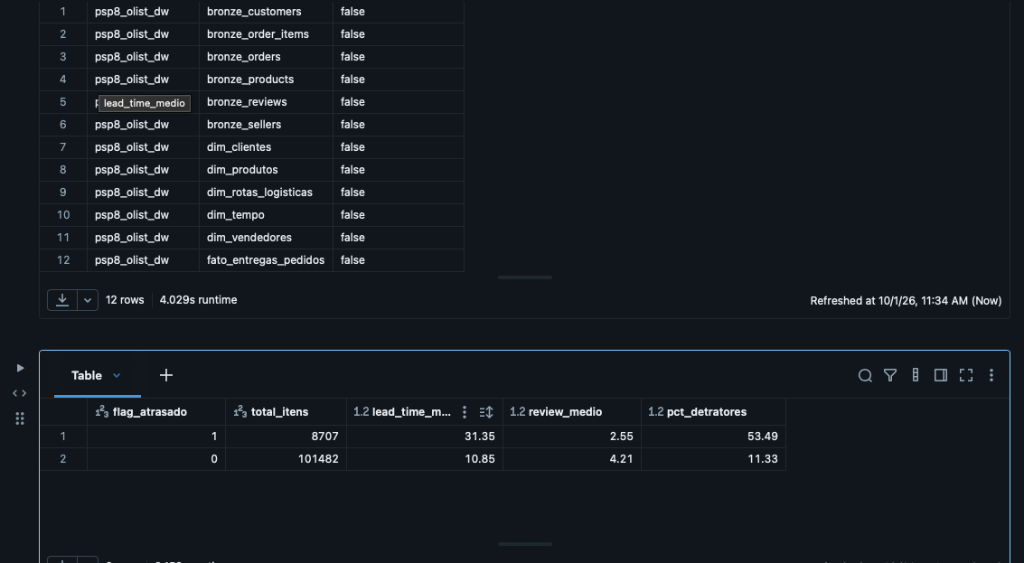
\includegraphics[width=0.96\columnwidth,height=4.2cm,keepaspectratio]{figuras/02_execucao_pipeline_etl_nuvem.png}
\caption{Validação do Pipeline Medalhão e Persistência das Tabelas Delta no Databricks.}
\label{fig:pipeline_databricks}
\end{figure}

\subsection{Formulação Matemática e Métricas Operacionais}
Para garantir rigor formal e reprodutibilidade científica, definem-se os operadores e funções matemáticas que regem as métricas do SAD:

\subsubsection{Lead Time Real de Entrega \texorpdfstring{($LT_i$)}{(LTi)}}
Mede a duração temporal efetiva, expressa em dias decimais, transcorrida entre o instante de compra ($t_{\text{compra}, i}$) e a data física de recebimento confirmada pelo cliente ($t_{\text{entrega}, i}$):
\begin{equation}
LT_i = \frac{t_{\text{entrega}, i} - t_{\text{compra}, i}}{86.400}
\label{eq:lead_time}
\end{equation}
onde o denominador $86.400$ converte os carimbos em segundos para dias solares completos.

\subsubsection{Prazo Prometido pela Plataforma \texorpdfstring{($PE_i$)}{(PEi)}}
Representa a expectativa contratual informada ao consumidor no ato do fechamento do pedido:
\begin{equation}
PE_i = \frac{t_{\text{estimada}, i} - t_{\text{compra}, i}}{86.400}
\label{eq:prazo_prometido}
\end{equation}

\subsubsection{Desvio de Prazo Operacional \texorpdfstring{($\Delta_i$)}{(Delta i)}}
Diferença algébrica entre a data real de recebimento e o prazo contratado:
\begin{equation}
\Delta_i = \frac{t_{\text{entrega}, i} - t_{\text{estimada}, i}}{86.400} = LT_i - PE_i
\label{eq:desvio_prazo}
\end{equation}

\subsubsection{Indicador Binário de Atraso \texorpdfstring{($\mathbb{I}_{\text{atrasado}, i}$)}{(I atrasado)}}
Função indicadora booleana de descumprimento do prazo prometido:
\begin{equation}
\mathbb{I}_{\text{atrasado}, i} = \begin{cases} 
1, & \text{se } \Delta_i > 0 \\ 
0, & \text{se } \Delta_i \le 0 
\end{cases}
\label{eq:flag_atraso}
\end{equation}

\subsubsection{Indicador de Atraso Crítico \texorpdfstring{($\mathbb{I}_{\text{grave}, i}$)}{(I grave)}}
Classifica ocorrências operacionais que superam $48\text{ horas}$ de atraso relativo ao prazo limite contratado:
\begin{equation}
\mathbb{I}_{\text{grave}, i} = \begin{cases} 
1, & \text{se } \Delta_i > 2{,}0\text{ dias} \\ 
0, & \text{se } \Delta_i \le 2{,}0\text{ dias} 
\end{cases}
\label{eq:flag_atraso_grave}
\end{equation}

\subsubsection{Razão de Carga Logística / Burden \texorpdfstring{($\mathcal{B}_i$)}{(Bi)}}
Razão adimensional que quantifica o peso financeiro do frete ($V_{\text{frete}, i}$) em relação ao valor de venda do item ($V_{\text{preço}, i}$):
\begin{equation}
\mathcal{B}_i = \frac{V_{\text{frete}, i}}{V_{\text{preço}, i}}
\label{eq:burden}
\end{equation}

\subsubsection{Indicador de Cliente Detrator \texorpdfstring{($\mathbb{I}_{\text{detrator}, i}$)}{(I detrator)}}
Em conformidade com a teoria clássica de satisfação e fidelização \citep{reichheld2003one}, clientes que atribuem notas $1$ ou $2$ na escala discreta de avaliação $S_i \in \{1, 2, 3, 4, 5\}$ são formalmente categorizados como detratores:
\begin{equation}
\mathbb{I}_{\text{detrator}, i} = \begin{cases} 
1, & \text{se } S_i \in \{1, 2\} \\ 
0, & \text{se } S_i \in \{3, 4, 5\} 
\end{cases}
\label{eq:flag_detrator}
\end{equation}

\subsubsection{Taxa Agregada de Atrasos \texorpdfstring{($\tau_k$)}{(tau k)}}
A taxa percentual de atrasos para qualquer subconjunto amostral $\mathcal{S}_k \subset \mathcal{S}$ (por exemplo, uma região geográfica ou rota específica) é calculada pela média amostral do indicador de atraso:
\begin{equation}
\tau_k = \left( \frac{1}{|\mathcal{S}_k|} \sum_{i \in \mathcal{S}_k} \mathbb{I}_{\text{atrasado}, i} \right) \times 100\%
\label{eq:taxa_atraso}
\end{equation}

\subsubsection{Modelo Matemático de Simulação de CSAT \texorpdfstring{($\overline{S}_{\text{sim}}$)}{(S sim)}}
Para quantificar o benefício gerencial de programas de redução de falhas logísticas, desenvolveu-se um modelo de sensibilidade que estima a nova nota média geral de satisfação caso uma fração $\alpha \in [0, 1]$ dos pedidos atrasados fosse entregue dentro do prazo contratado:
\begin{align}
\overline{S}_{\text{sim}}(\alpha) = \frac{1}{N_{\text{total}}} \Big[ &(N_{\text{pont}} + \alpha N_{\text{atra}}) \cdot \overline{S}_{\text{pont}} \nonumber \\
&+ ((1 - \alpha) N_{\text{atra}}) \cdot \overline{S}_{\text{atra}} \Big]
\label{eq:simulacao_csat}
\end{align}
onde $N_{\text{pont}}$ e $N_{\text{atra}}$ representam o número total de itens pontuais e atrasados na base histórica, $\overline{S}_{\text{pont}}$ e $\overline{S}_{\text{atra}}$ correspondem às respectivas médias observadas de nota de avaliação, e $N_{\text{total}} = N_{\text{pont}} + N_{\text{atra}}$.

% --- 3. RESULTADOS E DISCUSSÃO ---
\section{Resultados e Discussão}
\label{sec:resultados}

A aplicação dos operadores matemáticos sobre o Esquema Estrela Delta Lake gerou as respostas quantitativas para as cinco questões de negócio formuladas.

\subsection{P1: Disparidade Regional no Lead Time e Atrasos}
A análise comparativa do desempenho das entregas entre as cinco macrorregiões brasileiras evidenciou uma profunda assimetria territorial (Tabela~\ref{tab:regional} e Figura~\ref{fig:regional}).

\begin{table*}[t]
\centering
\small
\caption{Desempenho Logístico de Entrega no E-Commerce por Macrorregião de Destino}
\label{tab:regional}
\resizebox{\textwidth}{!}{%
\begin{tabular}{lccccc}
\toprule
\textbf{Região de Destino} & \textbf{Total de Itens} & \textbf{Lead Time Médio (Dias)} & \textbf{Lead Time Mediana (Dias)} & \textbf{Prazo Prometido Médio (Dias)} & \textbf{Taxa de Atraso (\%)} \\
\midrule
Norte        & $2.148$  & 22,59 & 20,16 & 32,83 & 9,80\% \\
Nordeste     & $10.840$ & 20,01 & 17,32 & 30,11 & 14,33\% \\
Centro-Oeste & $6.480$  & 15,02 & 13,28 & 24,67 & 7,97\% \\
Sul          & $15.545$ & 14,03 & 12,12 & 23,48 & 7,05\% \\
Sudeste      & $75.176$ & 10,75 & 8,71  & 22,23 & 7,45\% \\
\bottomrule
\end{tabular}%
}
\end{table*}

\begin{figure}[htbp]
\centering
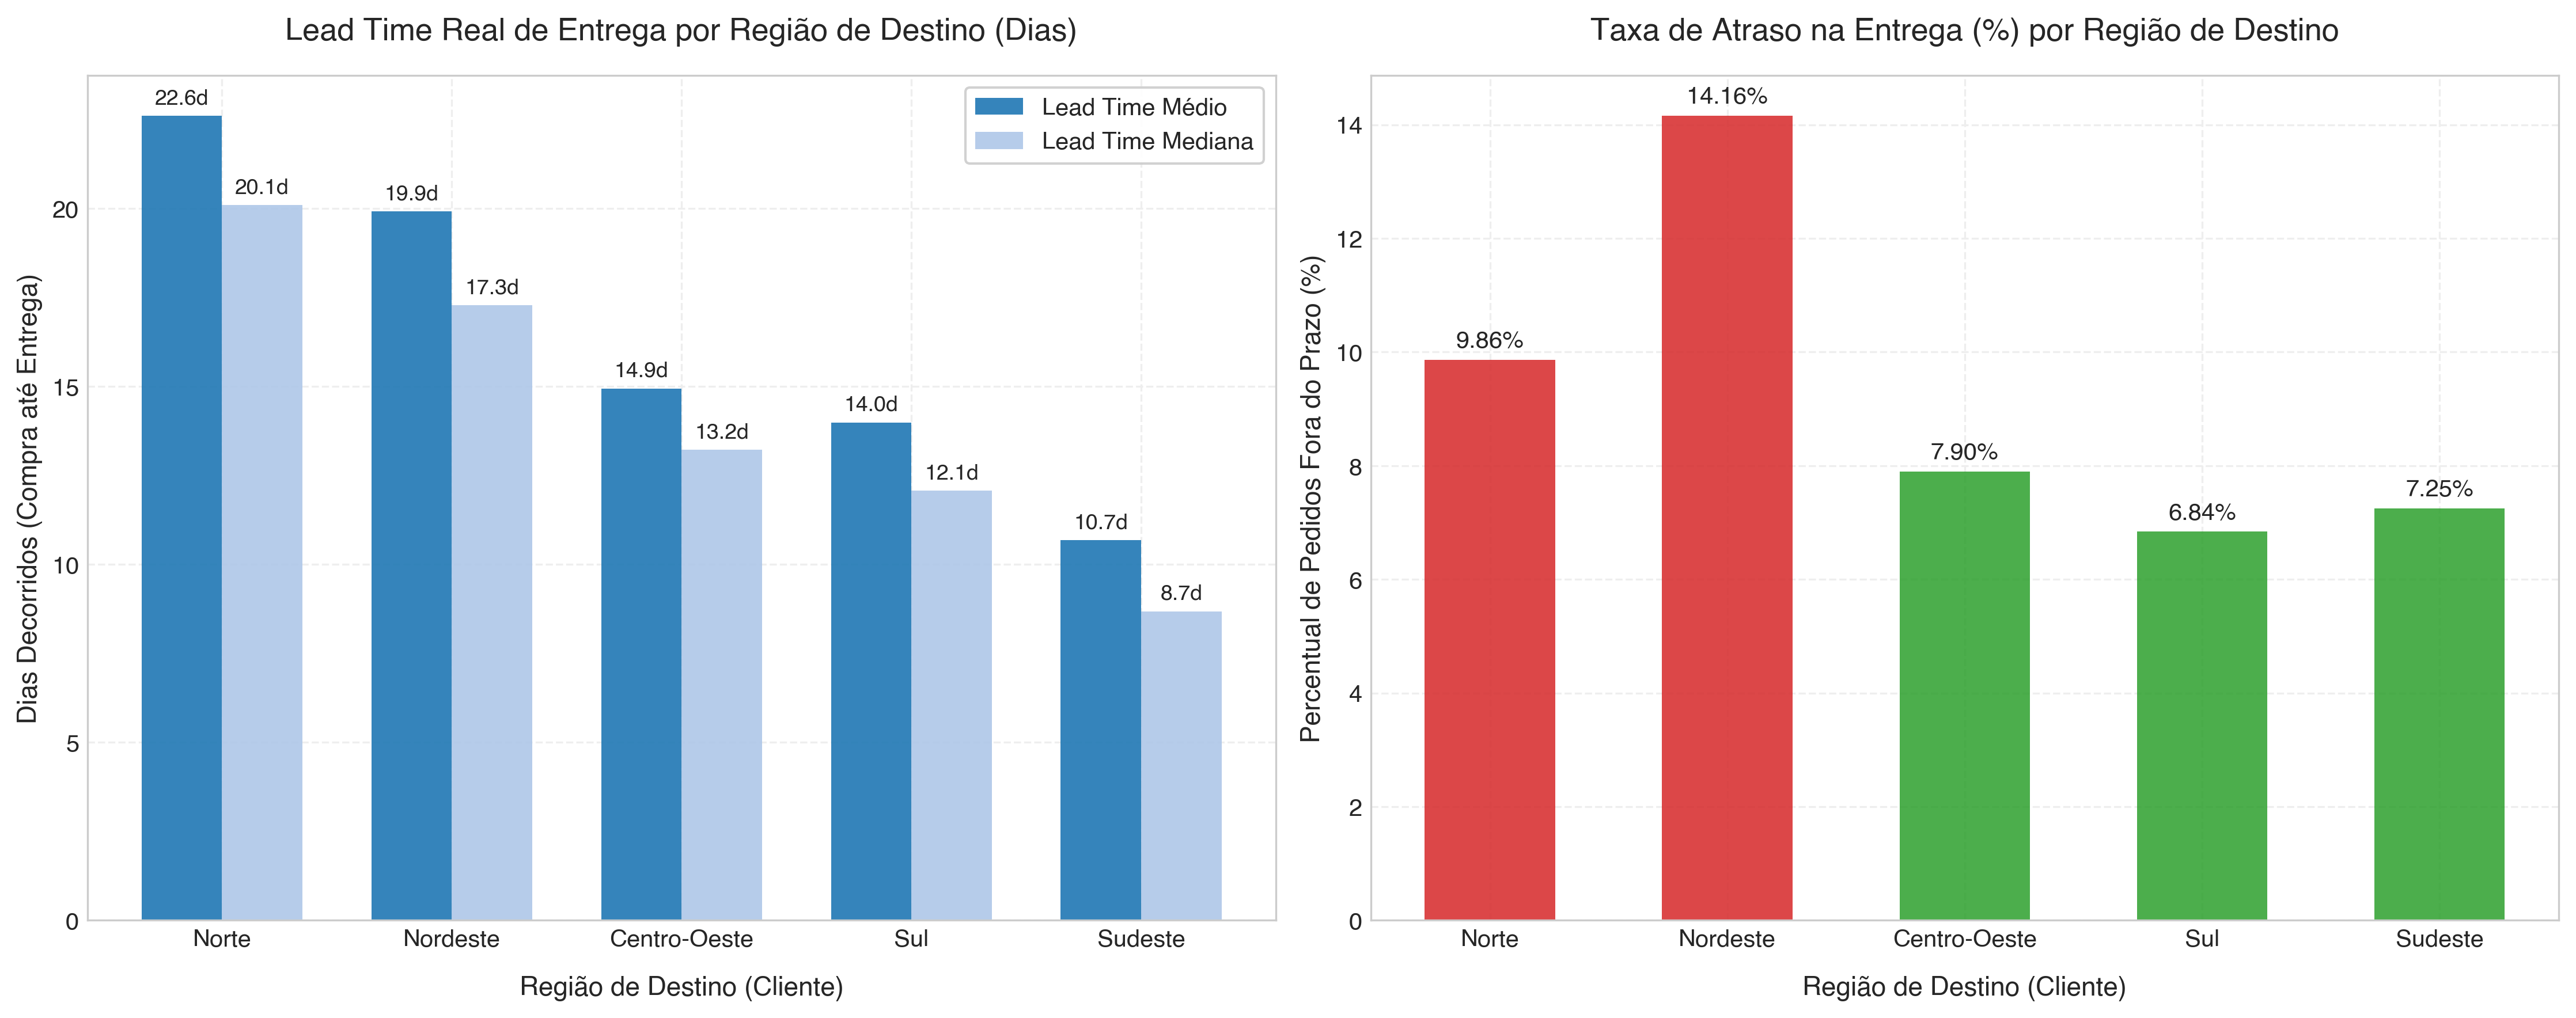
\includegraphics[width=0.96\columnwidth,height=4.6cm,keepaspectratio]{figuras/01_disparidade_regional_lead_time.png}
\caption{Disparidade no \textit{Lead Time} Real e Taxa de Atraso por Região.}
\label{fig:regional}
\end{figure}

Os dados atestam que, enquanto um comprador no Sudeste aguarda em média $10,75\text{ dias}$ (mediana de $8,71\text{ dias}$), o consumidor da Região Norte espera em média $22,59\text{ dias}$ para receber sua compra — um tempo mais de duas vezes superior. 

O ponto de maior vulnerabilidade operacional, entretanto, reside na Região Nordeste: além de um \textit{lead time} médio severamente alongado ($20,01\text{ dias}$), o Nordeste exibe a maior taxa de atraso de todo o território nacional ($\tau_{\text{Nordeste}} = 14,33\%$). Em termos empíricos, um em cada sete pedidos entregues na região extrapola a data limite prometida pela plataforma. 

A inspeção da dispersão e variabilidade através do gráfico de boxplot (Figura~\ref{fig:boxplot_regional}) revela que as distribuições do Norte e Nordeste apresentam caudas superiores extremamente longas, evidenciando instabilidade operacional decorrente de restrições de infraestrutura rodoviária e complexidade nas etapas de transferência inter-regional \citep{oliveira2022desafios}.

\begin{figure}[htbp]
\centering
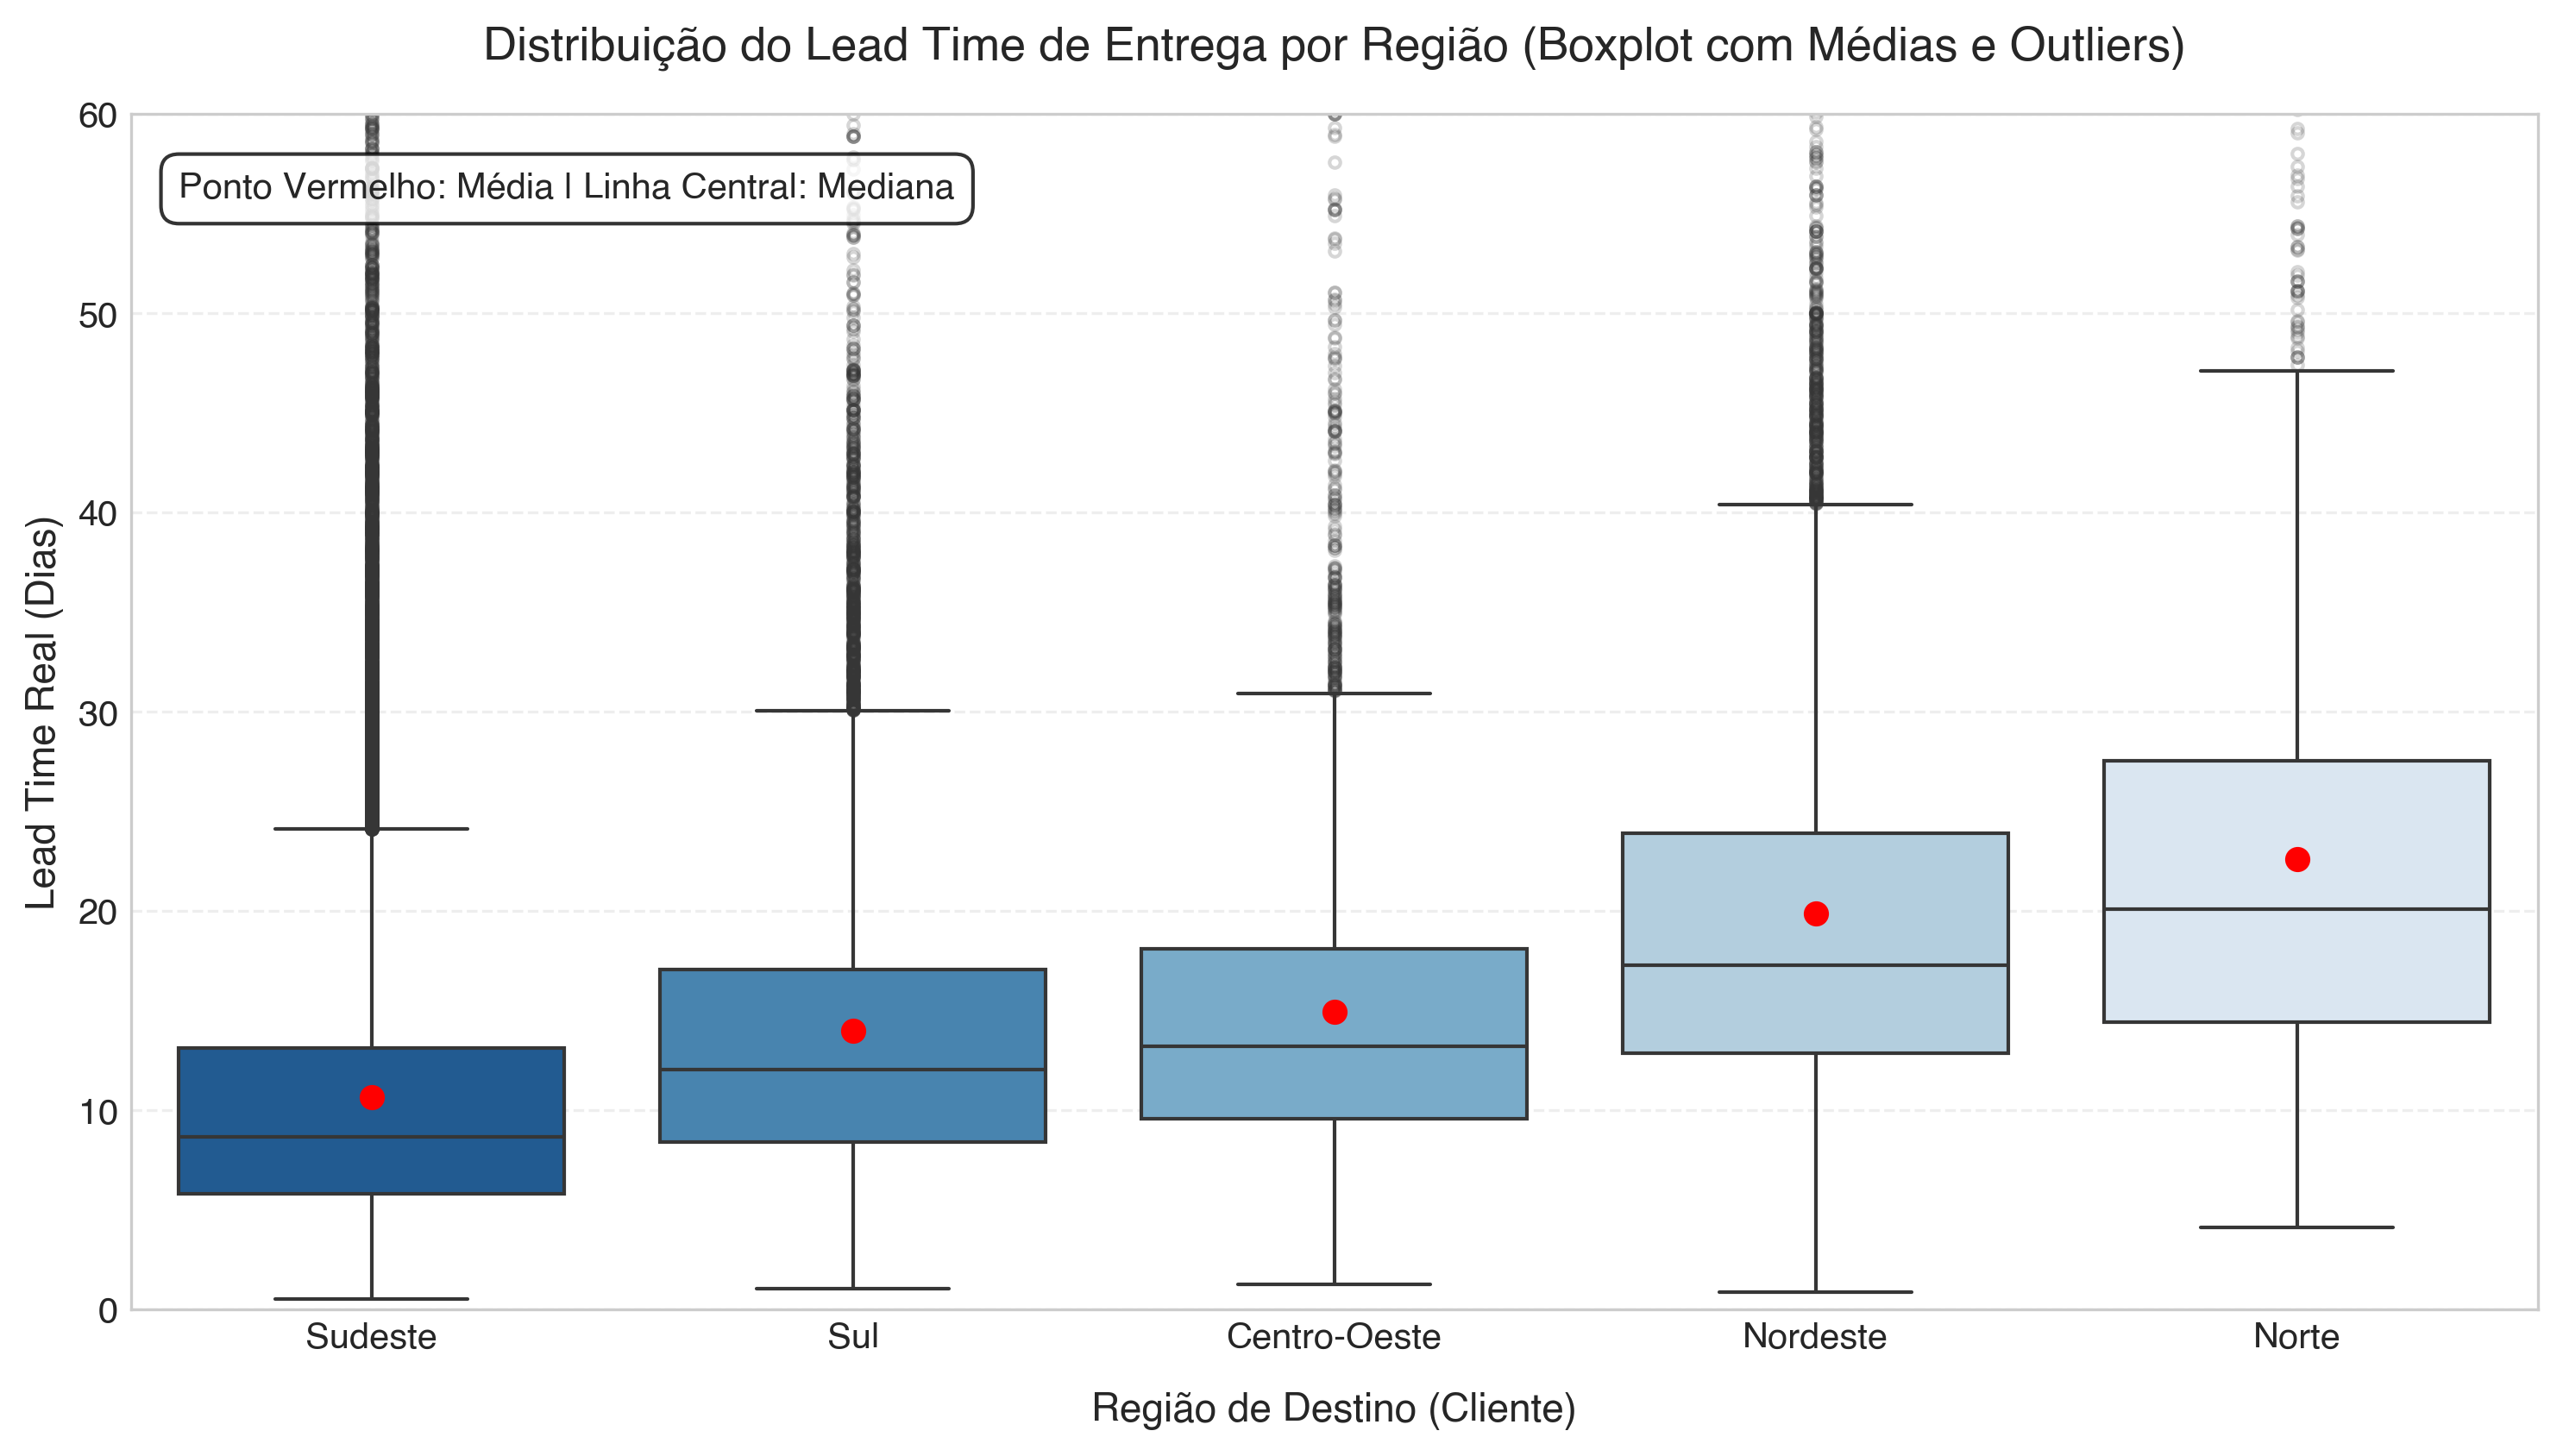
\includegraphics[width=0.96\columnwidth,height=4.4cm,keepaspectratio]{figuras/02_boxplot_lead_time_regiao.png}
\caption{Boxplot Comparativo da Dispersão do \textit{Lead Time} por Região de Destino.}
\label{fig:boxplot_regional}
\end{figure}

\subsection{P2: Razão Frete/Preço (Burden) vs. Satisfação}
A avaliação do peso relativo do frete ($\mathcal{B}_i$) sobre a nota média e a formação de clientes detratores revelou uma relação estatística direta entre onerosidade logística e rigor de avaliação (Tabela~\ref{tab:burden} e Figura~\ref{fig:burden}).

\begin{table}[htbp]
\centering
\caption{Relação entre a Razão Frete/Preço e Indicadores de Nível de Serviço}
\label{tab:burden}
\resizebox{\columnwidth}{!}{%
\begin{tabular}{lcccc}
\toprule
\textbf{Faixa de Frete/Preço ($\mathcal{B}$)} & \textbf{Total Itens} & \textbf{Score Médio} & \textbf{\% Detratores} & \textbf{Taxa Atraso} \\
\midrule
$< 10\%$                  & $30.803$ & 4,26 & 8,7\%  & 7,1\% \\
$10\%$ a $20\%$           & $37.075$ & 4,22          & 9,6\%           & 7,7\% \\
$20\%$ a $35\%$           & $25.138$ & 4,14          & 10,8\%          & 8,5\% \\
$35\%$ a $50\%$           & $9.822$  & 4,05          & 12,4\%          & 8,9\% \\
$50\%$ a $100\%$          & $5.765$  & 3,96          & 13,8\%          & 9,2\% \\
$> 100\%$ (Frete $>$ Item) & $1.586$  & 3,92 & 14,8\% & 9,5\% \\
\bottomrule
\end{tabular}%
}
\end{table}

\begin{figure}[htbp]
\centering
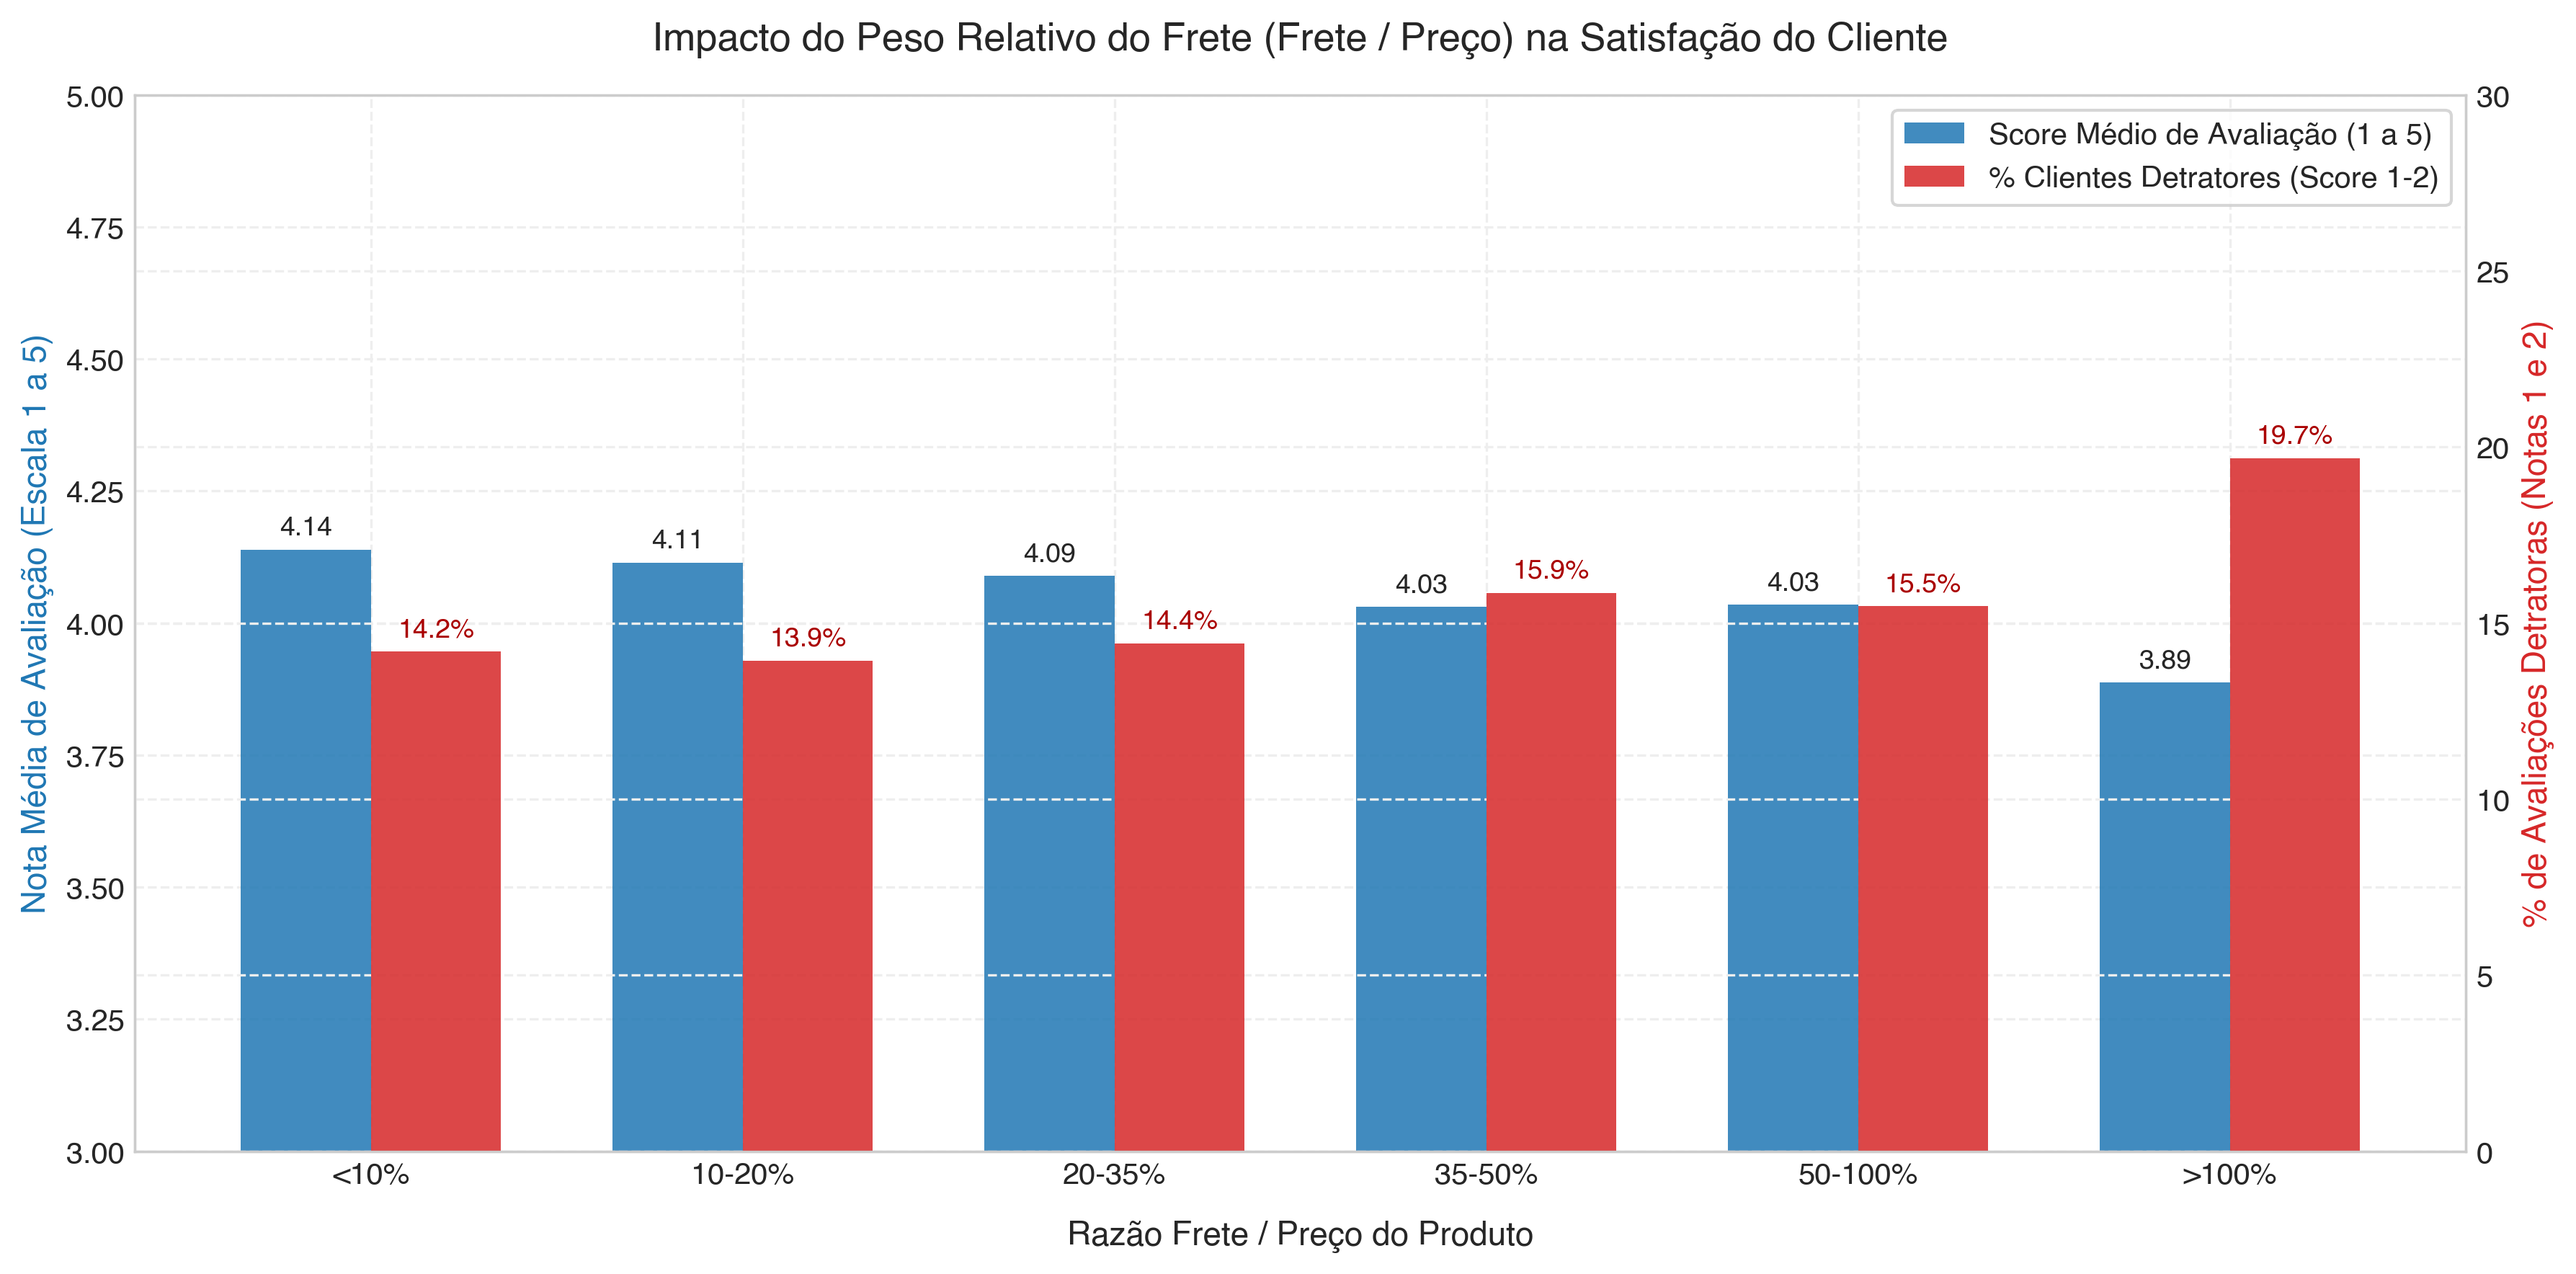
\includegraphics[width=0.96\columnwidth,height=4.4cm,keepaspectratio]{figuras/03_burden_frete_vs_satisfacao.png}
\caption{Degradação da Satisfação do Consumidor em Função do \textit{Burden} de Frete.}
\label{fig:burden}
\end{figure}

Observa-se uma deterioração monotônica e estrita no nível de serviço percebido à medida que o frete se torna proporcionalmente oneroso. Em compras nas quais o frete custa mais que o próprio item transacionado ($\mathcal{B}_i > 100\%$), a proporção de clientes detratores praticamente dobra, saltando de $8,7\%$ para $14,8\%$, enquanto a nota média declina de $4,26$ para $3,92$. Conforme preconizado por \citet{silva2023gestao}, o frete elevado altera a ancoragem psicológica do consumidor, elevando sua exigência de perfeição e tornando-o intolerante a qualquer atrito na entrega.

\subsection{P3: Gargalos Operacionais por Categoria de Produto}
A estratificação do desempenho de entrega para categorias mercadológicas com volume representativo ($\ge 500$ itens comercializados) demonstrou que o perfil físico e dimensional dos produtos é fator determinante nos prazos (Figura~\ref{fig:categorias}).

\begin{figure}[htbp]
\centering
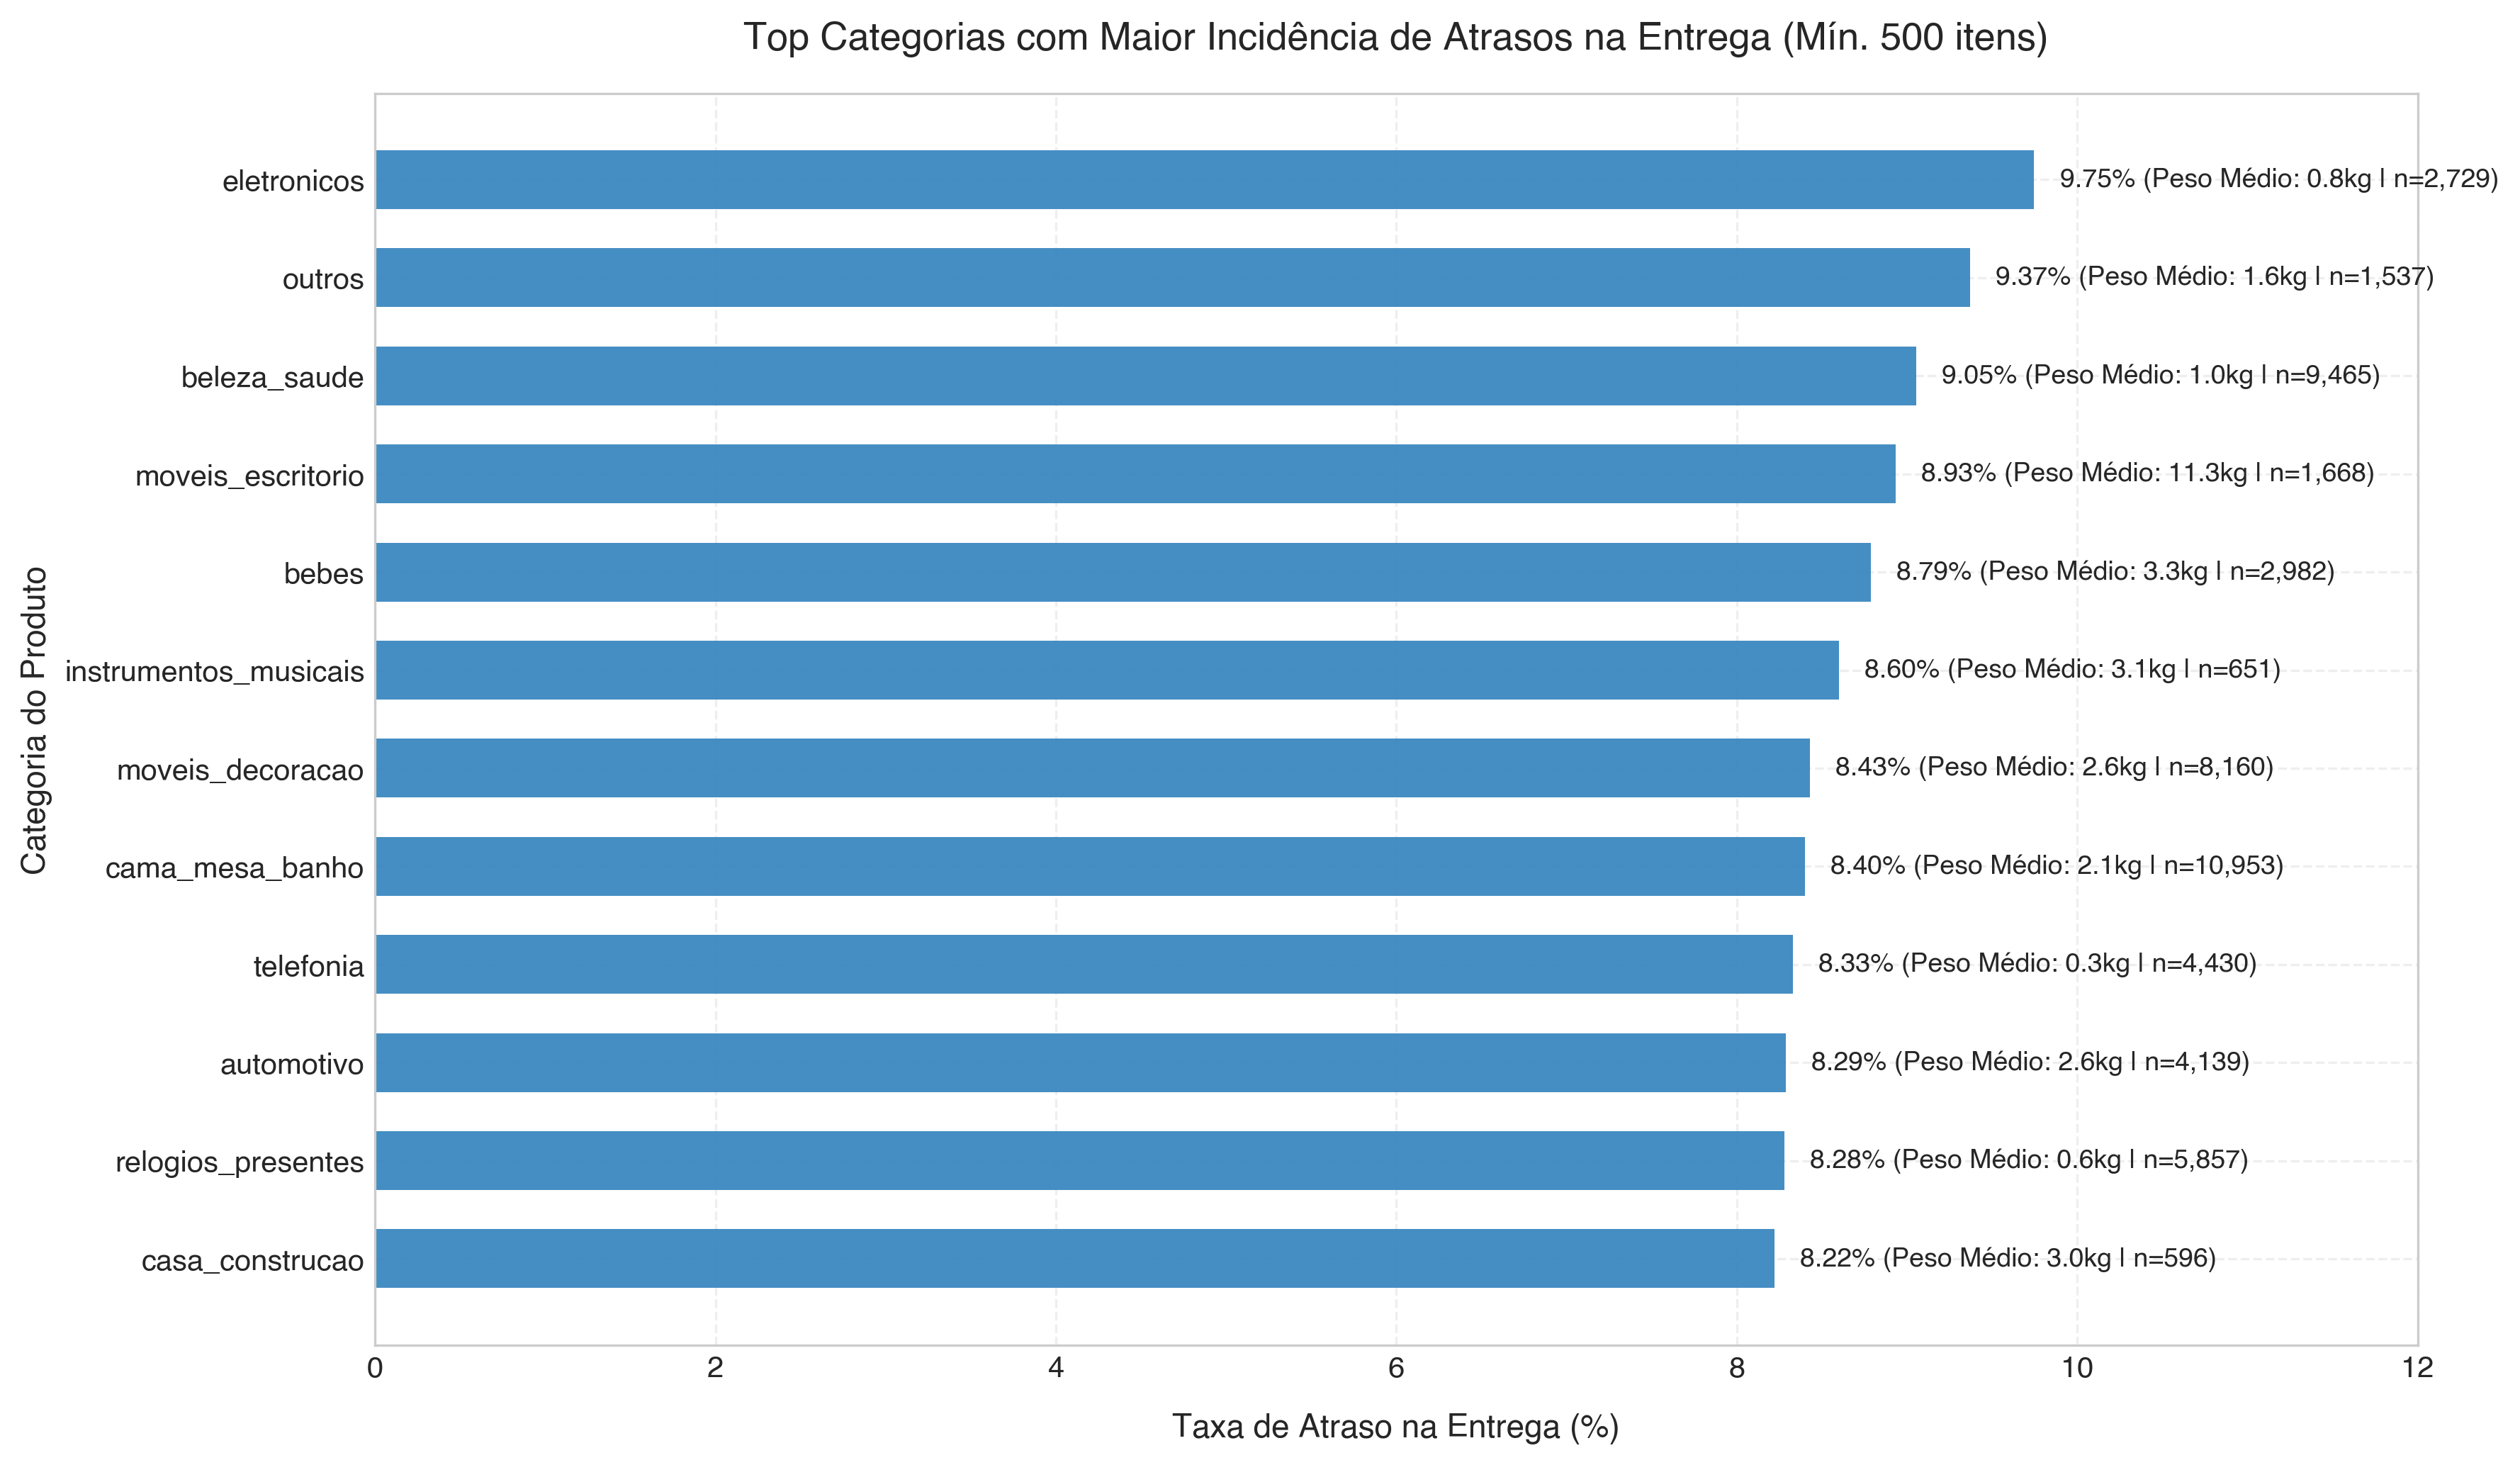
\includegraphics[width=0.96\columnwidth,height=4.5cm,keepaspectratio]{figuras/04_top_categorias_atraso.png}
\caption{Categorias com Maior Taxa de Atraso e Associação com Cubagem e Massa.}
\label{fig:categorias}
\end{figure}

As maiores incidências de atrasos concentram-se em mercadorias de elevada cubagem e massa bruta, com destaque para a categoria de móveis de escritório (\textit{office furniture}), que registra taxa de atraso de $8,93\%$ e peso médio de $11,3\text{ kg}$, e artigos eletrônicos ($9,75\%$). Móveis exigem manuseio específico e transporte por malhas rodoviárias de carga fracionada pesada (\textit{Less-Than-Truckload} - LTL), sujeitas a menor frequência de despachos e maiores dificuldades de descarregamento em perímetros urbanos adensados \citep{matos2025,novaes2007logistica}.

\subsection{P4: Complexidade de Rota e Atrasos Severos}
Ao categorizar a malha logística segundo a complexidade dos arcos geográficos de transporte (Tabela~\ref{tab:rotas} e Figura~\ref{fig:rotas_matriz}), comprova-se o impacto da transposição de divisas estaduais na estabilidade do serviço.

\begin{table}[htbp]
\centering
\caption{Desempenho Logístico por Tipologia de Rota}
\label{tab:rotas}
\resizebox{\columnwidth}{!}{%
\begin{tabular}{lcccc}
\toprule
\textbf{Tipologia de Rota} & \textbf{Volume Itens} & \textbf{Taxa Atraso} & \textbf{Atraso $>48$h} & \textbf{Frete Médio} \\
\midrule
1. Intraestadual          & $39.549$ & 6,06\% & 3,68\% & R\$ 13,53 \\
2. Interestadual (Região) & $28.790$ & 9,78\% & 7,69\% & R\$ 20,85 \\
3. Inter-regional         & $41.850$ & 8,91\% & 6,82\% & R\$ 25,99 \\
\bottomrule
\end{tabular}%
}
\end{table}

\begin{figure}[htbp]
\centering
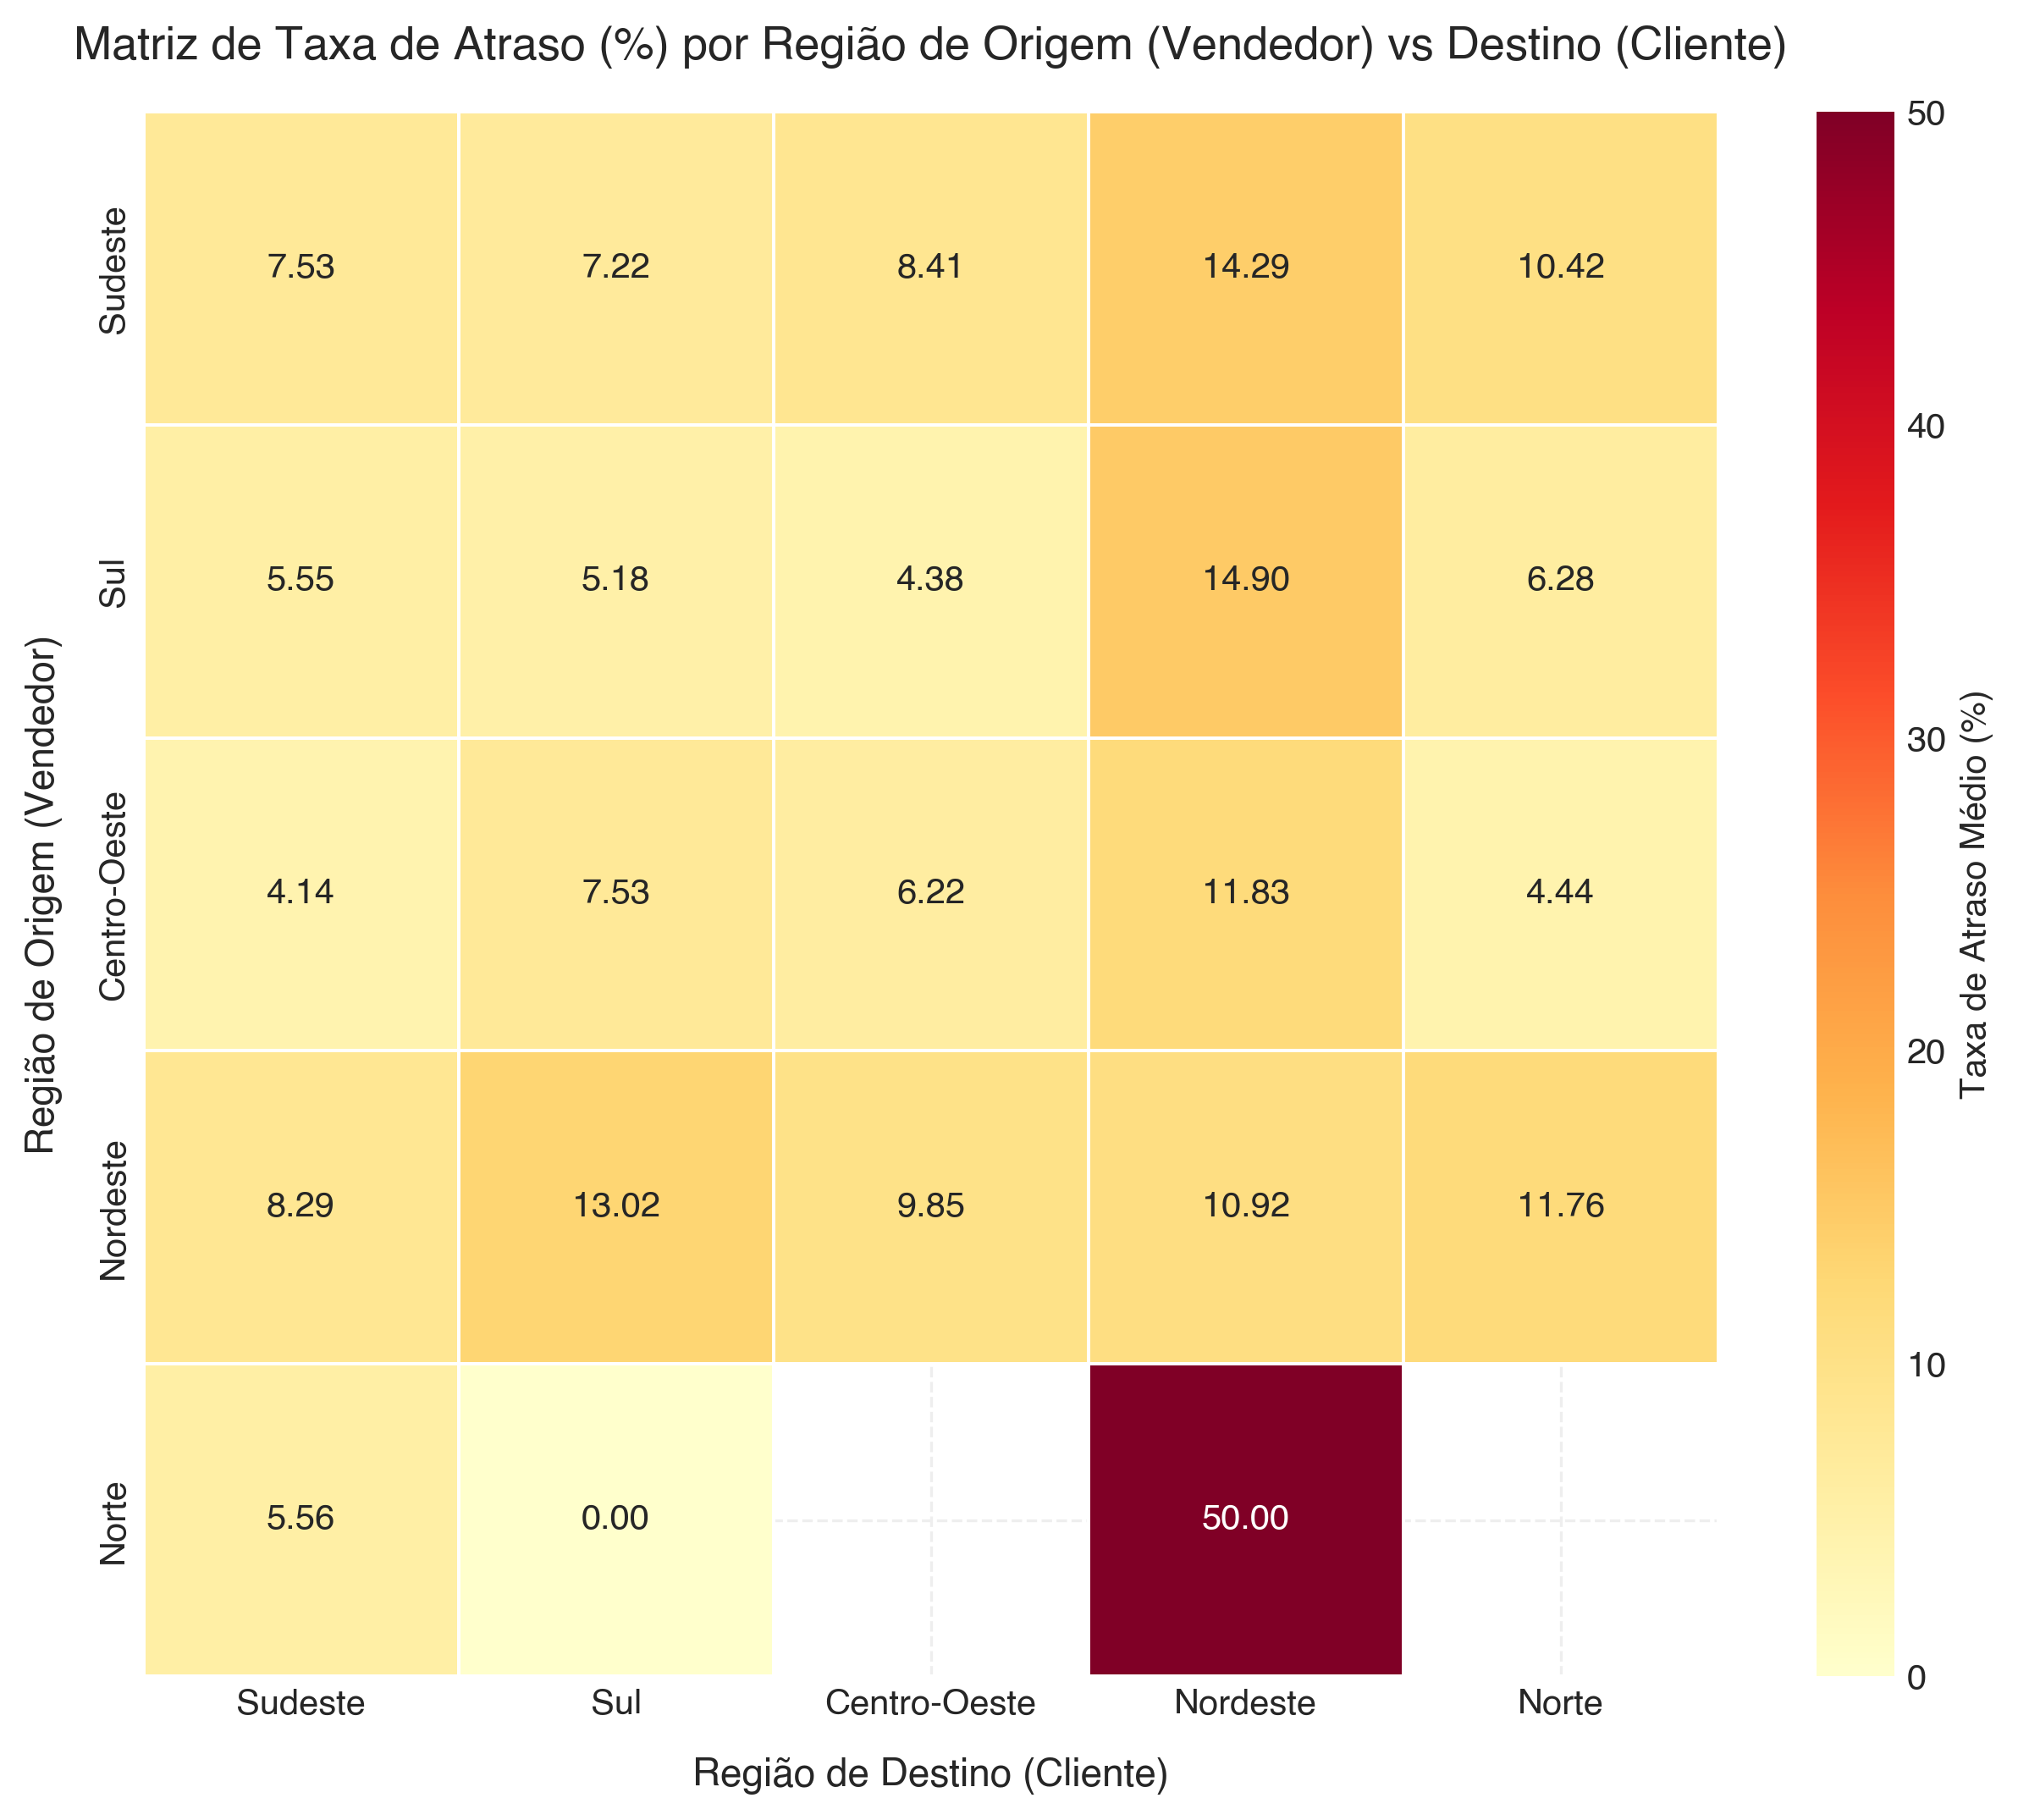
\includegraphics[width=0.96\columnwidth,height=4.5cm,keepaspectratio]{figuras/05_matriz_rotas_taxa_atraso.png}
\caption{Matriz de Atrasos Logísticos Cruzando Macrorregiões de Origem e Destino.}
\label{fig:rotas_matriz}
\end{figure}

Entregas realizadas no mesmo estado de expedição (rotas intraestaduais) apresentam controle operacional robusto, registrando apenas $3,68\%$ de atrasos severos ($> 48\text{ horas}$). Contudo, nas rotas que atravessam fronteiras estaduais, a probabilidade de atrasos graves salta para $7,69\%$ — mais que o dobro. A análise da matriz origem-destino revela que os fluxos inter-regionais que partem dos polos vendedores do Sudeste e Sul com destino ao Nordeste apresentam taxas de atraso sistematicamente superiores a $14\%$ e $15\%$, apontando gargalos severos de consolidação, transbordo e transferência em rodovias interestaduais \citep{oliveira2022desafios}.

\subsection{P5: Impacto do Atraso no CSAT e Modelo de Simulação}
O cruzamento das métricas operacionais de pontualidade com as avaliações dos clientes comprovou o impacto decisivo do cumprimento de prazos na satisfação do usuário (Tabela~\ref{tab:atraso_csat} e Figura~\ref{fig:csat}).

\begin{table}[htbp]
\centering
\caption{Impacto do Cumprimento de Prazos na Satisfação do Consumidor}
\label{tab:atraso_csat}
\resizebox{\columnwidth}{!}{%
\begin{tabular}{lcccc}
\toprule
\textbf{Status da Entrega} & \textbf{Avaliações} & \textbf{Nota Média} & \textbf{Mediana} & \textbf{\% Detratores} \\
\midrule
Entrega no Prazo ($\mathbb{I}_{\text{atra}} = 0$)   & $88.163$ & 4,29 & 5,0 & 9,21\% \\
Entrega com Atraso ($\mathbb{I}_{\text{atra}} = 1$) & $7.661$  & 2,56 & 2,0 & 54,07\% \\
\bottomrule
\end{tabular}%
}
\end{table}

\begin{figure}[htbp]
\centering
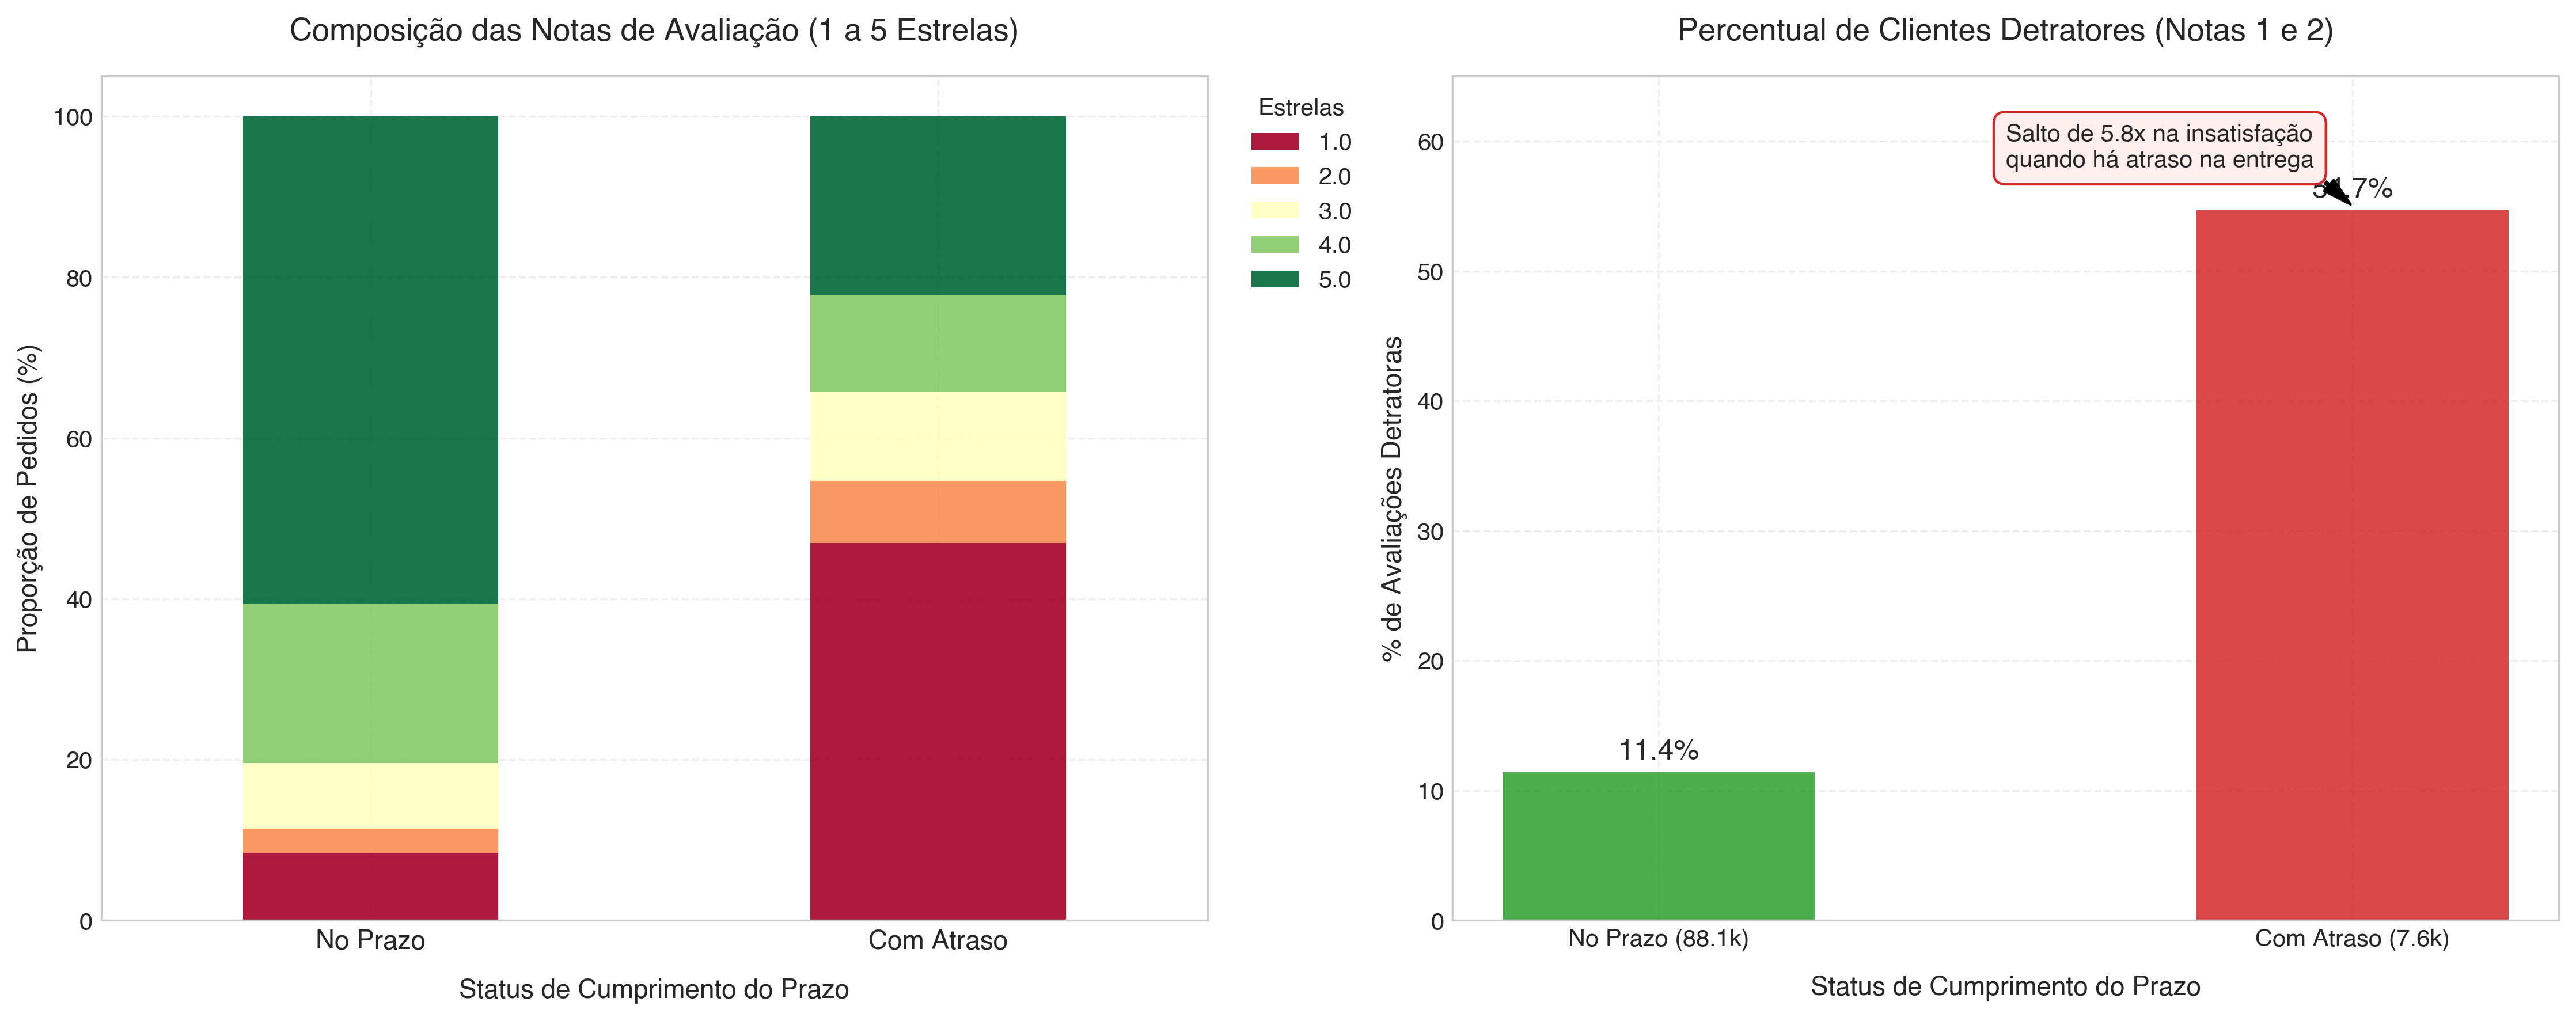
\includegraphics[width=0.96\columnwidth,height=4.4cm,keepaspectratio]{figuras/06_impacto_atraso_csat.png}
\caption{Distribuição de Notas e Incidência de Detratores em Função do Atraso.}
\label{fig:csat}
\end{figure}

O descumprimento do prazo contratual manifestou-se como o elemento isolado de maior poder destrutivo da reputação do serviço: em entregas pontuais, a nota média atinge $4,29$ estrelas, e a proporção de detratores é de apenas $9,21\%$. Quando ocorre atraso, a nota média despenca para $2,56$ estrelas, e o percentual de detratores atinge impressionantes $54,07\%$ — uma amplificação de 5,8 vezes.

Aplicando-se a formulação de simulação de sensibilidade da Equação~\ref{eq:simulacao_csat} com redução de $50\%$ nas falhas de prazo ($\alpha = 0{,}5$):
\begin{align*}
N_{\text{pont}} &= 88.163, \quad \overline{S}_{\text{pont}} = 4,2953 \\
N_{\text{atra}} &= 7.661, \quad \overline{S}_{\text{atra}} = 2,5634 \\
N_{\text{total}} &= 95.824
\end{align*}
A nota média global da plataforma se elevaria de $\overline{S} = 4,1568$ para $\overline{S}_{\text{sim}}(0{,}5) = 4,2260$, representando um ganho sustentável de $+0,07$ pontos em toda a base e resgatando mais de $3.800$ consumidores da categoria de detratores, o que se traduz em substancial redução de custos com atendimento ao cliente e contenção de \textit{churn} \citep{reichheld2003one,sucena2023}.

\subsection{Diretrizes Prescritivas para a Tomada de Decisão}
Com base no diagnóstico empírico, propõem-se quatro diretrizes estratégicas para gestores de operações e logística no comércio eletrônico brasileiro:
\begin{enumerate}
    \item \textit{Descentralização de estoques no Nordeste}: A elevada incidência de atrasos ($14,33\%$) nos fluxos com destino ao Nordeste exige a instalação de centros de consolidação e estoques avançados (\textit{micro-hubs}) nas regiões metropolitanas de Recife e Salvador, convertendo fretes rodoviários interestaduais de longo curso em saídas de distribuição de última milha locais \citep{matos2025}.
    \item \textit{Segmentação operacional por cubagem}: Mercadorias volumosas e de alta densidade (como móveis) demandam contratos de transporte dedicados à carga fracionada pesada e vitrines com janelas de prazo prometido calibradas para evitar expectativas irrealistas no ato da compra.
    \item \textit{Políticas dinâmicas de subsídio e teto de frete}: Para conter a formação de detratores em transações cujo frete supera o preço do produto ($\mathcal{B} > 100\%$), recomenda-se a aplicação de tetos dinâmicos de frete subsidiados pela plataforma ou incentivos ao agrupamento de pedidos (\textit{bundling}).
    \item \textit{Mecanismo preditivo de alerta prévio}: Incorporação de modelos de aprendizado supervisionado (\textit{Machine Learning}) acoplados à esteira de checkout para estimar, no instante da compra, o risco de estouro de prazo com base na rota e características do produto, permitindo a seleção preventiva de modais mais ágeis.
\end{enumerate}

% --- 4. CONCLUSÃO ---
\section{Conclusão}
\label{sec:conclusao}
O presente trabalho demonstrou que o desenvolvimento de Sistemas de Apoio à Decisão ancorados em infraestruturas distribuídas em nuvem (\textit{Databricks / Delta Lake}) constitui ferramenta indispensável para o diagnóstico e mitigação de ineficiências na logística de distribuição do comércio eletrônico nacional. Apoiando-se no processo formal de KDD e no modelo dimensional de Ralph Kimball, a pesquisa quantificou e modelou matematicamente os fatores críticos que condicionam o nível de serviço ao consumidor.

As evidências empíricas atestaram que o atraso na entrega é o principal vetor de degradação da experiência do cliente, multiplicando por $5,8$ vezes a taxa de clientes detratores e evidenciando a extrema vulnerabilidade da cadeia de suprimentos em rotas interestaduais com destino ao Nordeste. A simulação matemática comprovou que intervenções logísticas focadas na redução de metade dos atrasos são capazes de resgatar milhares de clientes insatisfeitos e elevar a percepção de valor geral da plataforma.

Como limitações da investigação, destaca-se a ausência de identificação nominal das transportadoras executoras no conjunto de dados público da Olist, o que impossibilitou um \textit{benchmarking} concorrencial direto, e a representação geoespacial truncada pelo prefixo do CEP. Para trabalhos futuros, recomenda-se a integração de fluxos contínuos de eventos via \textit{Delta Live Tables} e o treinamento de algoritmos de aprendizado de máquina supervisionados para a predição antecipada de atrasos operacionais no instante do fechamento da compra.

% --- REFERÊNCIAS BIBLIOGRÁFICAS ---
\begingroup
\small
\setlength{\bibsep}{2.0pt plus 0.5pt}
\bibliographystyle{plainnat}
\bibliography{referencias}
\endgroup

\end{document}
